\section{Entanglement and Operator Spreading in Quantum Circuits} \label{sec:circuits}

One drawback to studying systems with time-independent Hamiltonians is that their dynamics are constrained by their conservation laws~\cite{Jonay18}. Systems with no conservation laws would not have these constraints. Quantum circuits have no explicit Hamiltonian, but rather evolve unitarily at discrete time steps. 

The circuits provide solvable systems in certain limits, after averaging over circuit architecture. In this limit, which will be discussed later in this section, it is easier to discuss information dynamics in terms of entanglement entropy rather than operator spreading. This is not to say that operator spreading does not apply in circuits, or that entanglement dynamics do not apply to Hamiltonian systems. Rather, this is an easier tool to use for these systems.

In this section we first introduce bitartite entanglement entropy and the constraints it must satisfy. We then discuss the construction of quantum circuits, and the behavior of the entanglement entropy in these circuits. We show that it is possible to calculate $v_B$ entirely from the entanglement entropy, and that this velocity is the same as $v_B$ calculated from operator spreading.

\subsection{Entanglement Entropy} \label{sub:intro}

Quantum entanglement has applications to branches of physics from high energy and quantum information theory to experimental studies of cold atomic gases. Although entanglement is so widely studied, its dynamics are less well understood. The dynamics of the entanglement are closely related to the speed at which information travels or spreads. 

Let us briefly review entanglement in composite systems. First assume the full system $AB$ can be decomposed into subsystems $A$ and $B$, and $AB$ is in the pure state $\ket{\Psi}_{{AB}}$. In the spin chains considered here, the chain is often divided such that $A$ is all spins on one side of a cut and $B$ is all spins on the other side. Another common decomposition is having $A$ be all spins between two cuts, and $B$ being all other spins. If the states of $A$ and $B$ are entangled it is impossible to write $\ket{\Psi}_{AB} = \ket{\psi_A}_A \ket{\psi_B}_B$. If this is possible then $\ket{\Psi_{{AB}}}$ is called a product state. Subscripts on kets represent the space that the ket lives in, but this is clear from the name of the state (uppercase for the full state, subscripts otherwise) so we will drop the outside subscripts.

We can assess the amount of entanglement by looking at the density matrix $\rho_{AB} = \ket{\Psi}\bra{\Psi}$. All density matrices satisfy $\Tr \rho = 1$. Generic pure state density matrices further satisfy 
\begin{align}
\Tr \rho^2 = \Tr\ket{\psi}\bra{\psi}\ket{\psi}\bra{\psi} = \Tr\ket{\psi}\bra{\psi} = 1.
\end{align}
We can further construct the reduced density matrices $\rho_A$ and $\rho_B$ as the full density matrix $\rho_{AB}$ traced over subsystem $B$ and $A$, respectively. If $\ket{\Psi}$ is a product state, the reduced density matrices are $\rho_A = \ket{\psi_A}\bra{\psi_A}$, etc. However, if the states are entangled the reduced density matrices do not have such a nice form. They will still have trace 1, but $\Tr\rho^2<1$ for a mixed state.

A maximally entangled state will be of the form
\begin{align}
\ket{\Psi} = \sum_i^N\th{\sqrt{N}}\ket{\psi_{A,i}}\ket{\psi_{B,i}},
\end{align}
where $N$ is the dimension of the larger of the two Hilbert spaces and $i$ labels orthogonal states. $\Tr\rho_{AB}^2=1$ because the full state is pure. The reduced density matrices are
\begin{align}
\rho_A = \sum_i^N\th{N}\ket{\psi_{A,i}}\bra{\psi_{A,i}},
\end{align}
with $\Tr\rho_A^2 = \sum_i\th{N^2}=\th{N}$, with similar results for $B$. This provides the constraints $\th{N}\le\Tr\rho^2\le 1$. 

Bipartite entanglement entropy provides a more general way to quantify the entanglement and is defined as the quantum entropy of one of the reduced density matrices. As long as the full state is pure, this is equivalent for either subsystem. There are multiple quantum entropies. The $n$th Renyi entropy of density matrix $\rho$ is 
\begin{align}
S_n = \th{1-n}\log\left(\Tr\rho^n\right). \label{eqn:renyi}
\end{align}
In the limit $n\to1$ this becomes the von Neumann entropy 
\begin{align}
S_{vN} &= \th{1-(1+\epsilon)}\log\left(\Tr\rho^{1+\epsilon}\right) \nn
&= -\frac{1}{\epsilon}\log \Tr \rho \rho^{\epsilon}\nn
&= -\th{\epsilon}\log\Tr\rho\left(1+\epsilon\rho\right) \nn
&= -\Tr\rho\log\rho,
\end{align}
the analogue of the classical Shannon entropy. The calculation uses the small $x$ expansions of $a^x$ and $\log(1+x)$. All Renyi entropies are maximized by maximally mixed states, with entropy $N\log q$ for $N$-site systems with $q$-dimensional Hilbert spaces at each site. They are also minimized by pure states, which have entropy 0.

For the spin chain, we can define many different subsystems, each with a corresponding entanglement entropy. The following description is largely taken from~\cite{Nahum2017}. Consider a spin chain of N sites with dimension $q$. Sites are labeled by $i=1,\dots N$, while the bonds between sites are labeled by $x = 1,\dots N-1$. After cutting the system at bond $x$, define the entropy across this cut as the bipartite entanglement entropy of all sites to the right of $x$. If the whole chain is in a pure state, this is equal to the bipartite entanglement entropy of all sites to the left of $x$.

We can define a function $S(x) = -\Tr\rho_x\log\rho_x$ where $\rho_x$ is the density matrix of the system with all sites left of $x$ traced out. As long as the full system is in a pure state, this is the von Neumann entanglement entropy of the two subsystems divided by the bond at $x$. For convenience logarithms are taken base $q$. $S(x)$ will observe constraints not already made clear due to the fact that subsystems defined by adjacent $x$ have heavy overlap.

Classically, for an arbitrary system decomposable into subsystems $A$ and $B$, the entropies satisfy $\max(S(A), S(B)) \leq S(AB)\leq S(A) + S(B)$. In quantum mechanics, this is replaced by the subadditivity of the von Neumann entropy 
\begin{align}
\left|S(A)-S(B)\right| \leq S(AB)\leq S(A) + S(B). \label{eqn:subadd}
\end{align}
If we take subsystem $A$ to be the single site between cuts $x$ and $x+1$ and subsystem $B$ to be all sites right of $x+1$, this becomes
\begin{align}
\left|S_1 - S(x+1)\right| \leq S(x) \leq S_1 + S(x+1),
\end{align}
where $S_1$ denotes the entropy of the single site between cuts $x$ and $x+1$. After some rearranging this can be written $\left|S(x+1) - S(x)\right| \leq S_1$. However, since the single site is $q$ dimensional, $S_1 \leq \log_q q = 1$, explaining the use of $q$ for the base. The preceding arguments taken together give the constraint
\begin{align}
\left|S(x+1) - S(x)\right| \leq 1. \label{eqn:offbyone}
\end{align}

A finite system has $S(x)$ pinned at its endpoint, because the entanglement entropy of a single site is bounded by 1. Then the maximally entangled state has $S(x) = \min\{x,L-x\}$. As the entanglement approaches this value it takes forms as in Fig.~\ref{fig:Tower}.
\begin{figure}
	\centering
	\includegraphics[width=.5\linewidth]{Tower}
	\caption{\textbf{Bitartite entanglement entropy at different times,} ($t = 340$, 690, 1024, 1365, 1707, 2048 and 4096). This data comes from a circuit model, but the behavior is believed to be general. Figure from~\cite{Nahum2017}.}
	\label{fig:Tower}
\end{figure}
The flat section has a constant growth rate $\pd{S(x,t)}{t}$ so the border position $y$ moves at a constant speed defined by the growth rate and the slope. Since the maximal slope is $\pd{S(x,t)}{x}=1$, this velocity is
\begin{align}
\pd{y}{t} = \pd{S}{t}\left(\pd{S}{x}\right)^{-1} = \pd{S}{t} = v_E. 
\label{eqn:vE}
\end{align}
This entanglement speed is equivalent to \_\_\_\_\_\_\_\_\_\_

Refs.~\cite{Keyserlingk, Jonay17, Jonay18, Nahum2017} discuss the speed of entanglement in brickwork models using related concepts called out of time order commutator (OTOC) and operator density. Reference~\cite{Zhou2017} quantifies the scrambling using the operator entanglement entropy opEE of the time evolution operator.

\subsection{Circuit Architectures} \label{sub:arch}

Like the earlier systems, quantum circuits consist of chains of Hilbert spaces. Instead of evolving under a time-independent Hamiltonian, they evolve with unitary operators, called gates, at discrete times. If a gate acts on a site at time $t$ it is said to `fall' on that site. Simple circuits only contain 2-site gates which act on the product of Hilbert spaces at adjacent sites. There is a possibility of confusion regarding the term ``operator": the ``unitary operator," ``unitary gate," or just ``gate" will be the time evolution operator of the circuit, while ``operator" without qualification will refer to the observable that is evolving in time.

We could study the dynamics of a single circuit, in analogy with the single Hamiltonian studied in the previous section. However, it is also instructive to look at ensembles of circuits, with some type of randomness. This section presents two sources of randomness, the choice of gates and their locations in the circuit.

%References~\cite{Keyserlingk} and~\cite{Nahum2017} both discuss circuits of this type. Both discuss random circuits, although with different sources of randomness. 
One source is the unitary operator chosen at each site at each time. Different gates result in different architectures. 
If the Hilbert space at each site is $q$ dimensional, the space of 2-site unitary matrices is $q^2\times q^2$ dimensional. To find representative behavior, each circuit is made by drawing gates from some distribution. The circuits can then be averaged over these choices. A common choice is the Haar distribution, which is invariant to rotations in the space of 2-site operators. Since these act on a $q^2$-dimensional Hilbert space, there are $q^4$ independent operators, including one trivial operator (the identity). 

Another source of randomness is the placement of the gates. The ``brickwork" model~\cite{Keyserlingk} uses a deterministic architecture, in which at odd times there is a gate to the right of every odd site, while for even times there is a gate to the right of every even site. Figure~\ref{fig:brickcircuit} shows an example. The ``random" architecture~\cite{Nahum2017} chooses a random site for a single gate at each time step $t = n/\gamma$, where $\gamma$ is the gate rate and $n$ is an integer. The placement is then averaged over. 

\begin{figure}
	\centering
	\input{brickcircuit}
	\caption{\textbf{Brickwork circuit architecture}. The red circles represent the initial states of the system, while the blue rectangles are unitary gates that evolve the system in time. The Hilbert space at each site is $q$-dimensional, meaning the gates are $q^2\times q^2$ unitary  matrices, chosen from the Haar distribution. Adapted from~\cite{Keyserlingk}.}
	\label{fig:brickcircuit}
\end{figure}

The random architecture is equivalent to placing gates at each site in continuous time with Poisson-distributed time steps, as the gate rate $\gamma$ and the length $L$ are taken to infinity with the gate rate density $\gamma/L$ held constant.~\cite{Nahum2017}. This thesis focuses on a generalization of this model, described in Sec.~\ref{sec:stairs}.

%At least say that large $q$ moves operator ends to the right with probability 1: this will be useful in discussing $v_B$.

We want to know how the Pauli end-weight $W(t,i)$ evolves in time in these circuits. Recall that, given an observable $\cal{O}(t)$ evolving in time, this measure how far $\cal{O}$ has spread. Consider a unitary gate falling on sites $i$ and $i+1$. Some components of the operator $\cal{O}(t)$ will be non-identity at site $i$ but identities after $i$, and will have weight $W(t, i)$ by definition. There are $q^2-1$ operators like this. A randomly chosen unitary gate will evolve the operator on sites $i$ and $i+1$ to a random operator that is not the identity on both sites. There are $q^4-1$ of these, $q^2-1$ of which are identities on the second site.

If some component of the observable ends on site $i+1$, the unitary can move the end back, if it evolves the observable at $i+1$ to the identity. Again, $q^2-1$ of the random final operators are identities on the second site, so that the probability of moving weight from site $i+1$ to $i$ is the same as not moving the weight from $i$ to $i+1$. The probability that a random gate advances $W(t,i)$ is $p = \frac{q^2}{q^2+1}$, so that $1-p = \frac{1}{q^2+1}$. After averaging over the possible circuits, this leads to the dynamics of $W(t,i)$, from~\cite{Keyserlingk}
\begin{align}
W(t+1, i) = (1-p)\left(W(t, i) + W(t, i+1)\right)\nn
W(t+1, i+1), = p\left(W(t, i) + W(t, i+1)\right). \label{eqn:opsp}
\end{align}
%
%[\emph{How much more detail should I go into before this just becomes a synopsis of their paper?}]
%
%The butterfly speed is
%\begin{align}
%v_B= \frac{q^2-1}{q^2+1}. \label{eqn:keysvb}
%\end{align}
%The entanglement speed is 
%\begin{align}
%v_E = \frac{\log\frac{q+q^{-1}}{2}}{\log q} = \frac{\log\left(1-v_B^2
%	\right)}{\log\left(\frac{1-v_b}{1+v_B}\right)}.\label{eqn:keysve}
%\end{align}
%These speeds describe operator spreading represented in Fig.~\ref{fig:onesite_spreading}.
%\begin{figure}
%	\centering
%	\includegraphics[width=.5\linewidth]{onesite_spreading}
%	\caption{\textbf{Operator spreading in a brickwork circuit}. $\bar{\rho_R}$ is what is here called $W(t,i)$. From~\cite{Keyserlingk}.}
%	\label{fig:onesite_spreading}
%\end{figure}
%An initially local operator spreads with velocity $v_B$, and diffuses at a rate related to $v_E$. 

\subsection{Deterministic Limit}  \label{sub:determ}

Note the the dynamics in Eq.~\ref{eqn:opsp} are degenerate in the large $q$ limit to deterministic movement of end sites with the application of each gate. This implies that this limit may be interesting, and indeed it is. This is more easily seen by studying the entropy growth.

Recall the entropy bound from Eq.~\ref{eqn:offbyone}. This means that when a gate falls at bond $x$, the maximum entanglement possible across cut $x$ is 
\begin{align}
S(x) \le \min\left\lbrace S(x-1), S(x+1)\right\rbrace + 1, \nonumber
\end{align}
while the gate does not affect $S(x-1)$ or $S(x+1)$. It would be helpful to find a solvable limit of quantum circuits under which this inequality is saturated because it would completely specify the evolution of the entanglement. 

Such a limit is found by taking $q\to\infty$. Ref.~\cite{Nahum2017} includes a detailed proof, but the key is that all unitary gates that do not saturate the bound obey some polynomial equation, so these operators define a measure zero subset on the Haar distribution. We know then that, with probability 1, the random two-site gate will maximize bipartite entanglement entropy.

Taken together, these facts mean that after a gate across cut $x$, the new entanglement entropy is
\begin{align}
S(x, t+1) = \min\left\lbrace S(x-1, t), S(x+1, t)\right\rbrace + 1.
	\label{eqn:update}
\end{align}
Then if at any time $S(x,t)$ becomes integer valued at all $x$, it remains so for the rest of the evolution. There are a few pictures that make this integer-valued evolution more intuitive.

\subsubsection{Surface Growth Picture}  \label{subsub:surfgrowth}

One model for the entropy growth described above is the Tetris-like surface growth picture. Here, the entropy is represented by a piecewise-constant function with the height given by the entropy across each cut, as in Fig.~\ref{fig:tetris}, taken from \cite{Nahum2017}. 
\begin{figure}
	\centering
	\includegraphics[width=.5\textwidth]{tetris.pdf}
	\caption{\textbf{Tetris-like model for large-$q$ chain.} The gate at cut $x$ adds enough entropy so that $S(x)$ is one greater than either of its neighbors. Figure from~\cite{Nahum2017}.}
	\label{fig:tetris}
\end{figure}
In general, it is possible for the entropy across two adjacent cuts to be equal. However, Fig.~\ref{fig:applyingUnitary}, also from~\cite{Nahum2017}, shows that flat sections can be destroyed but not created. 
\begin{figure}
	\centering
	\includegraphics[width=.5\textwidth]{applyingUnitary.pdf}
	\caption{\textbf{Several possibilities for local changes} in the large $q$ model. If three adjacent cuts all have equal entropy, the two flat sections annihilate each other. There is no way to generate flat sections.}
	\label{fig:applyingUnitary}
\end{figure}

If the system has been evolving for a long time, then, it makes sense then to only consider states that have no flat sections, so that $S(x) = S(x-1)\pm1$ for all $x$. In this case, instead of a picture like Fig.~\ref{fig:tetris} it is possible to represent the entropy at each bond as a point, with a diagonal slope connecting bonds. The slope between cuts (at a site) will always be $\pm1$. Instead of $2\times1$ or $1\times1$ rectangles, the gates are then squares coming down point-first, as in Fig.~\ref{fig:diaggate}. 
\begin{figure}
	\centering
	\input{diaggate}
	\caption{\textbf{Another picture of the configuration in Fig.~\ref{fig:tetris}}. Here the cut positions are top or bottom vertices of the squares. On the left, the gate at time $t$ results in entropy growth at $x$ because at time $t-1$, $S(x-1) > S(x) < S(x+1)$. On the right the gate has no effect. Although $S(x) < S(x+1)$, the case $S(x) < S(x-1)$ is not satisfied. The bottom row of the picture is not made of squares because the state has been evolving for a long time.}
	\label{fig:diaggate}
\end{figure}
If the gate falls on a local minimum, it lifts the entropy at that bond. If the gate falls on a local maximum or a non-extremum it has no effect.

\emph{Check this paragraph}
In this picture, we can describe an entropy curve as a series of up and down steps, with each step defined at a site (between two cuts), For example, the initial state in Fig.~\ref{fig:diagstairs} would be $uuudduuduudddd$ and the final state would be $uuuduudududddd$. To make this look like a classical spin system (as in the Ising model), we can a state $s$, where $s_i$ is the local slope at site $i$, with $u\to1$ and $d\to-1$. For reference we quote results from systems like this
\begin{align}
uu
\end{align}

Explain how correlation constrains probabilities of all 2-site configurations.

\subsubsection{Minimal Cut Picture} \label{subsub:mincut}

Using the fact that a productive gate raises the entropy at a cut by 2, we can use another picture of the dynamics based on Fig.~\ref{fig:brickcircuit}. Assume the initial state is a product state so the entropy at each cut is initially 0 and evolve with a brickwork circuit. Then after one of the first gates (for example between $i=3$ and $i=4$) the entropy at that cut will become 1. After any of the subsequent gates the entropy at the affected cut increases by 2.

The minimal cut picture~\cite{Nahum2017} reproduces this behavior by considering cuts through the circuit, as in Fig.~\ref{fig:mincut}.
\begin{figure}
	\centering
	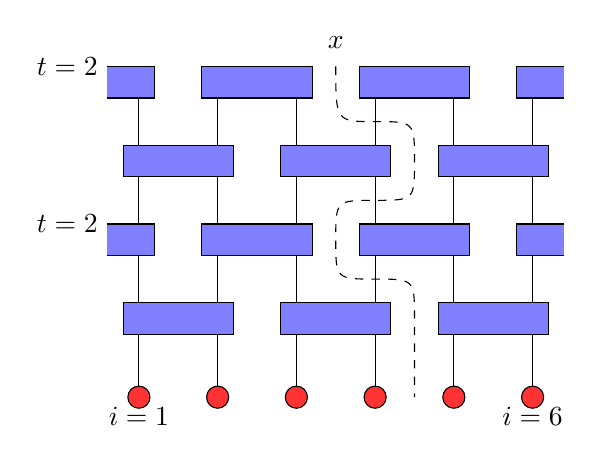
\begin{tikzpicture}[scale = 1]
\draw (0,0) node[below]{$i=1$} -- (0,4);
\filldraw[color=black, fill=red!80] (0,0) circle (4pt) node[anchor=west] { };
\draw (1,0) -- (1,4);
\filldraw[color=black, fill=red!80] (1,0) circle (4pt) node[anchor=west] { };
\draw (2,0) -- (2,4);
\filldraw[color=black, fill=red!80] (2,0) circle (4pt) node[anchor=west] { };
\draw (3,0) -- (3,4);
\filldraw[color=black, fill=red!80] (3,0) circle (4pt) node[anchor=west] { };
\draw (4,0) -- (4,4);
\filldraw[color=black, fill=red!80] (4,0) circle (4pt) node[anchor=west] { };
\draw (5,0) node[below]{$i=6$} -- (5,4);
\filldraw[color=black, fill=red!80] (5,0) circle (4pt) node[anchor=west] { };

\foreach \x/\y in {0/1, 2/1, 4/1, 1/2, 3/2, 0/3, 2/3, 4/3, 1/4, 3/4} 
\filldraw[color=black, fill=blue!50] (\x-.2,\y-.2) rectangle (\x+1.2,\y+.2);

\draw[fill=blue!50] (-.4,1.8) -- (.2,1.8) -- (.2,2.2) -- (-.4,2.2)
								node[left] {$t=2$};
\draw[fill=blue!50] (-.4,3.8) -- (.2,3.8) -- (.2,4.2) -- (-.4,4.2)
								node[left] {$t=2$};
\draw[fill=blue!50] (5.4,4.2) -- (4.8,4.2) -- (4.8,3.8) -- (5.4,3.8);
\draw[fill=blue!50] (5.4,2.2) -- (4.8,2.2) -- (4.8,1.8) -- (5.4,1.8);

\draw (2.5,4.5) node{$x$};
\draw[dashed] (2.5,4.2) .. controls (2.5,3.5) .. (3,3.5) 
                        .. controls (3.5,3.5) .. (3.5,3) 
                        .. controls (3.5,2.5) .. (3,2.5) 
                        .. controls (2.5,2.5) .. (2.5,2) 
                        .. controls (2.5,1.5) .. (3,1.5) 
                        .. controls (3.5,1.5) .. (3.5,1) 
                        .. controls (3.5,0.5) .. (3.5,0.5) 
                        .. controls (3.5,0.0) .. (3.5,0);
\end{tikzpicture}
	\caption{\textbf{Minimal cut picture.} Assuming an initial product state, $S(x)$ is given by the minimal number of legs that must be cut to draw a line from the bottom of the circuit to $x$. Cutting through gates is not allowed (or equivalently costs two cuts) and the initial point need not be $x$. Figure adapted from~\cite{Nahum2017}.}
	\label{fig:mincut}
\end{figure}
To find the entanglement across $x$, start in an unentangled state. If the initial state is entangled, include gates for $t<0$ that evolve a product state into the initial state at time $t=0$. Then, starting at the top of the circuit at $x$, find the path through the circuit that cuts through no gates and through the fewest of the lines defined by sites, called legs. The path need not end at $x$. The entanglement at $x$ is the number of legs cut by this path. 

For the brickwork circuit, this reproduces the entropy calculation quoted above, with first gates generating 1 unit of entanglement and subsequent gates generating 2. However, in circuits where not every gate is productive, the min-cut picture still works, and agrees with the surface growth picture.

Consider the circuit in Fig.~\ref{fig:degeneratemincut}.
\begin{figure}
	\centering
	\input{degeneratemincut}
	\caption{\textbf{Minimal cut with degenerate gates.} All gates at cut $x$ after the first gate there produce no entanglement because $S(x)$ is a local maximum.}
	\label{fig:degeneratemincut}
\end{figure}
After the initial gate acts between sites 3 and 4, $S(x)$ becomes a local maximum, with so that all gates after it become unproductive. In the surface growth picture this is represented by multiple gates falling on a local maximum. This is to show that the min-cut picture agrees with the surface growth picture, and provides another set of intuition for the dynamics of this class of circuits.

Since cuts through gates can considered as having cost 2, there is one more equivalent picture for the min-cut procedure: at the location of each gate, cross ("tangle") the two relevant strands. Fig.~\ref{fig:anothermincut} shows this picture for the same circuit as in Fig.~\ref{fig:degeneratemincut}.
\begin{figure}
	\centering
	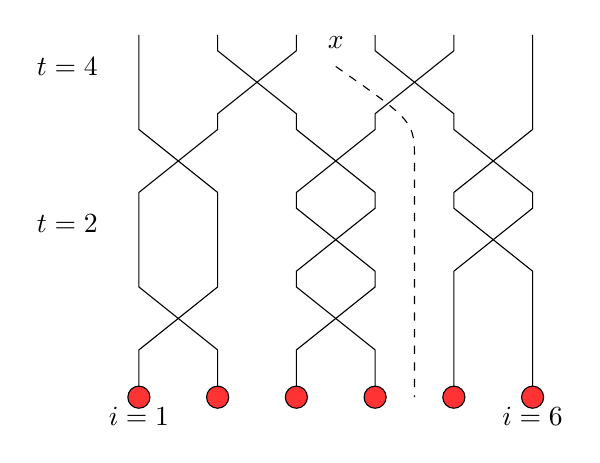
\begin{tikzpicture}[scale = 1]
\draw (0,0) node[below]{$i=1$} -- (0,.6) -- (1,1.4) -- (1,2.6) -- (0,3.4) -- (0,4.6);
\filldraw[color=black, fill=red!80] (0,0) circle (4pt) node[anchor=west] { };
\draw (1,0) -- (1,.6) -- (0,1.4) -- (0,2.6) -- (1,3.4) -- (1,3.6) -- (2,4.4) -- (2,4.6);
\filldraw[color=black, fill=red!80] (1,0) circle (4pt) node[anchor=west] { };
\draw (2,0) -- (2,.6) -- (3,1.4) -- (3,1.6) -- (2,2.4) -- (2,2.6) -- (3,3.4) -- (3,3.6) -- (4,4.4) -- (4,4.6);
\filldraw[color=black, fill=red!80] (2,0) circle (4pt) node[anchor=west] { };
\draw (3,0) -- (3,.6) -- (2,1.4) -- (2,1.6) -- (3,2.4) -- (3,2.6) -- (2,3.4) -- (2,3.6) -- (1,4.4) -- (1,4.6);
\filldraw[color=black, fill=red!80] (3,0) circle (4pt) node[anchor=west] { };
\draw (4,0) -- (4,1.6) -- (5,2.4) -- (5,2.6) -- (4,3.4) -- (4,3.6) -- (3,4.4) -- (3,4.6);
\filldraw[color=black, fill=red!80] (4,0) circle (4pt) node[anchor=west] { };
\draw (5,0) node[below]{$i=6$} -- (5,1.6) -- (4,2.4) -- (4,2.6) -- (5,3.4) -- (5,4.6);
\filldraw[color=black, fill=red!80] (5,0) circle (4pt) node[anchor=west] { };



\draw[fill=blue!50] (-.4,2.2) node[left] {$t=2$};
\draw[fill=blue!50] (-.4,4.2) node[left] {$t=4$};

\draw (2.5,4.5) node{$x$};
\draw [dashed] (2.5,4.2) .. controls (3.5,3.5) .. (3.5,3) 
                         .. controls (3.5,1.5) .. (3.5,1) 
                         .. controls (3.5,0.5) .. (3.5,0.5) 
                         .. controls (3.5,0.0) .. (3.5,0);
\end{tikzpicture}
	\caption{Another representation of the min-cut picture, with gates replaced by tangled strands. The advantage of this view is that gates clearly look like objects whose crossing has twice the cost of crossing a strand.}
	\label{fig:anothermincut}
\end{figure}

Instead of asking about the entanglement from $x$ to the bottom of the circuit, we can find the entanglement between $x$ and a specific bond position $y$ at the bottom of the circuit, where $x$ and $y$ are separated by time $t$. This is the entanglement of the time evolution operator $U(t)$, and will be denoted $S_U(y,x,t)$~\cite{Jonay18}. Then the entanglement is just the cost of the minimal cut from $x$ to $y$. There are two reasons this is a useful quantity. Once is in finding the entanglement of operators, as the space of operators behaves like a doubled space of state~\cite{Jonay17, Jonay18}. Alternatively, if we want to find $S(x)$ for an arbitrary initial entanglement, we can compute $S(x,y)$, and then $S(x) = \min_y\{S(x,y) + S_0(y)\}$.

\subsection{Coarse Graining and Long Wavelength Dynamics} \label{sub:coarse}

It is possible to abstract out even more of the detailed dynamics to consider the large scale behavior. To do this, interpret $S(x)$ as a continuous real valued function. The entanglement growth rate can be calculated under the assumption that up and down steps (from the picture in Fig.~\ref{fig:diaggate}) are uncorrelated and the large scale slope $\pd{S}{x}$ is constant. These assumptions hold only in the stead state of the random (1-stair) architecture. However, they are a useful first-order approximation to the behavior of other length stair circuits.

For an entropy surface with constant slope $m\equiv\pd{S}{x}$ and no correlations, each step from one site to the next has probability $\frac{1+m}{2}$ of being up and $\frac{1-m}{2}$ of being down. The assumption that there are no correlations is exact in the random architecture. Consider a gate operating on cut $x$ at time $t$. For the gate to increase the entropy $S(x)$, it must be the case that $S(x)<S(x-1), S(x+1)$. The probability of this is $\frac{1+m}{2} \frac{1-m}{2} = \frac{1-m^2}{4}$. In this case we have $S(x,t+1)=S(x,t)+2$, because the gate increases the entropy to be great than that of its neighbors. Then if the gates arrive at each cut with a rate $\gamma$, the entanglement growth rate is
\begin{align}
\pd{S}{t} = \gamma\frac{1-m^2}{2}\equiv \Gamma(m). \label{eqn:randomgrowthrate}
\end{align}
Useful checks of this formula are that the entropy does not increase at maximal or minimal slope $m=1,-1$, and that at $m=0$, $\pd{S}{t}=\gamma/2$, 1/4 the brickwork value. The latter rate makes sense because in the case of the brickwork circuit all gates are guaranteed to raise the entropy, while here only 1/4 will have an effect.

\subsubsection{Entanglement Velocity} \label{subsub:v_E }

$\Gamma(m)$ contains encodes a significant amount of information about the entanglement growth of the system~\cite{Jonay18}, and is useful in calculating both the entanglement velocity and the butterfly velocity. We will discuss this function in more detail and show how these speeds can be extracted.

Consider a linear section of the entanglement curve $S(x,t)$, and its evolution through time $\tau$. We know that $S(y,t+\tau) = \min_x\{S_U(y,x,\tau) + S(x,t)\}$. If we assume the gate architecture is translationally invariant (which is true in the large-scale limit) then $S_U(y,x,\tau)$ depends only on the slope $v = \frac{y-x}{\tau}$, multiplied by the length of the cut from $x$ to $y$. Graphically, this corresponds to Fig.~\ref{fig:legendre}.
\begin{figure}
	\centering
	\begin{tikzpicture}
\draw (0,0) node[left]{$t+\tau$} -- (8,0);
\draw (0,3) node[left]{$t$}      -- (8,3);
\draw (4,0) -- (7,3);
\draw (4,-.1) node[below]{$x = y-vt$} -- (4,.1);
\draw (7,2.9) -- (7,3.1) node[above]{$y$};
\draw (1,-.1) node[below]{$x = 0$} -- (1,.1);
\draw (7,-.1) node[below]{$x = y$} -- (7,.1);
\end{tikzpicture}
	\caption{\textbf{Graphical interpretation of the Legendre transform.} Since the architecture is spacially homogeneous, $S_U$ depends only on the length and slope of the cut and is $S_U(y,x,\tau) \equiv G(v)\tau$, where $v=(x-y)/\tau$}.
	\label{fig:legendre}
\end{figure}
Since we assumed the initial state was linear, we can write it as $S(x,t) = mx = mv\tau+my$. From the linearity of $S_U$, and the fact that its only other dependence is on $v$, we can define $S_U(y,x,\tau) \equiv G(v)\tau$. The final entanglement $S(y,t+\tau) = \min_x\{G(v)\tau + mv\tau\}$ can be differentiated with respect to $\tau$ to obtain.
\begin{align}
\Gamma(m) = \min_v\{G(v) + mv\}.
\end{align}
Ref.~\cite{Jonay18} contains this equation with an extra factor of $m_\text{eq}$, the equilibrium slope. In the large-$q$ random circuits we are considering, this slope is 1 due to the saturation of Eq.~\ref{eqn:offbyone}.

This formalism reproduces the calculation of the entanglement velocity in Eq.~\ref{eqn:vE}. The entanglement velocity is the speed at which the kinks between the flat section $m=0$ and the sloped sections $m=\pm1$ move in the coarse grained version of Fig.~\ref{fig:Tower}. The sloped section does not move up, while the flat section moves up at $\Gamma(0)$. To preserve the continuity of $S(x)$, the kinks have to move at $v_E=\Gamma(0)$. Fig.~\ref{fig:entanglevel} shows this calculation of $v_E$, and shows a similar calculation for the velocity of a kink between arbitrary slopes, as long as the kink is a local maximum.
\begin{figure}
	\centering
	\begin{tikzpicture}
\draw[->] (-.5,0) -- (5,0) node[below right]{$x$};
\draw[->] (0,-.5) -- (0,4) node[below left]{$S(x,t)$};
\draw[] (0,1) -- (3.5,1) -- (4.5,0);
\draw[->] (1,1.3) -- (1,2.2) ;
\draw (1.5,1.5) node{\small $\Gamma(0)$};
\draw (0,2.5) -- (2,2.5) -- (3.5,2.5);
\draw[dashed] (2,2.5) -- (3.5,1);
\draw[->] (3.2,3) -- (2,3) node[above right]{\small $v_E$};
\draw (4.5,.8) node{\small $m=-1$};
\draw (1.5,.7) node{\small $m=0$};
\end{tikzpicture}
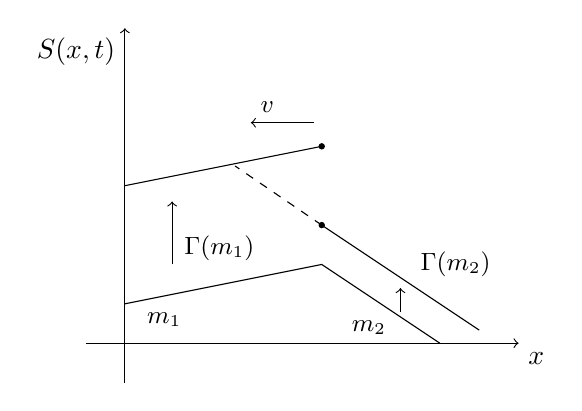
\begin{tikzpicture}
\draw[->] (-.5,0) -- (5,0) node[below right]{$x$};
\draw[->] (0,-.5) -- (0,4) node[below left]{$S(x,t)$};
\draw (0,0.5) -- (2.5,1) -- (4,0);
\draw (0,2) -- (2.5,2.5) node[draw,shape=circle, fill=black, scale=.2]{} (2.5,1.5) node[draw,shape=circle, fill=black, scale=.2]{} -- (4,.5) -- (4.5,.1666);
\draw[->] (.6,1) -- (.6,1.8) ;
\draw[->] (3.5,.4) -- (3.5,.7) ;
\draw (1.2,1.2) node{\small $\Gamma(m_1)$}
      (0.5,0.3) node{\small $m_1$}
      (4.2,1.0) node{\small $\Gamma(m_2)$}
      (3.1,0.2) node{\small $m_2$};
\draw[dashed] (2.5,1.5) -- (1.4,2.25);
\draw[->] (2.4,2.8) -- (1.6,2.8) node[above right]{\small $v$};
\end{tikzpicture}
	\caption{\textbf{Entanglement velocity in the surface growth picture.} The left figure shows a flat slope rising at $\Gamma(0)$. The right end is held down by the entanglement bounds. The dashed line shows the corrected $S(x)$. On the right both sections grow at the growth rates defined by their slopes. To maintain continuity the kink moves at $v=-\frac{\Gamma(m_2)-\Gamma(m_1)}{m_2-m_1}$.}
	\label{fig:entanglevel}
\end{figure}

The velocity between arbitrary slopes is $v = - \frac{\Gamma(m_2)-\Gamma(m_1)}{m_2-m_1}$, which has a nice interpretation in terms of the growth rate $\Gamma(m)$. This is the slope a chord drawn on the growth rate function between points corresponding to the two slopes, as in Fig.~\ref{fig:growthchord}.
\begin{figure}
	\centering
	\begin{tikzpicture}
\draw[->] (-3,0) -- (3,0) node[below right]{$m$};
\draw[->] (0,-.5) -- (0,3) node[below left]{$\Gamma(m)$};
\draw[domain=-2:2] plot (\x, {2-\x*\x/2});
\draw (-2,-.1) node[below]{\footnotesize $m=-1$} -- (-2,.1);
\draw (-2,0) -- (0,2);
\end{tikzpicture}
\quad
\begin{tikzpicture}
\draw[->] (-3,0) -- (3,0) node[below right]{$m$};
\draw[->] (0,-.5) -- (0,3) node[below left]{$\Gamma(m)$};
\draw[domain=-2:2] plot (\x, {2-\x*\x/2});
\draw (.4,-.1) node[below]{\footnotesize $m_1$} -- (.4,.1);
\draw (-.75,-.1) node[below]{\footnotesize $m_2$} -- (-.75,.1);
\draw (.4, 2-.4*.2) -- (-.75, 2-.75*.75/2);
\end{tikzpicture}
	\caption{\textbf{Calculation of kink speed from chord,} using the growth rate for random circuits, Eq.~\ref{eqn:randomgrowthrate}.Note that the chord slopes are positive, while the corresponding velocities (Fig.~\ref{fig:entanglevel}) are negative.}
	\label{fig:growthchord}
\end{figure}

\subsubsection{Butterfly Velocity} \label{subsub:v_B}

The same calculation does not work if the kink is a local minimum, as these feature diffuse. This is because a perturbation to the kink will travel up faster than either side of the kink, filling in the kink with a smooth curve. There is a well defined point where this curve hits the linear section with slope $m$ at a tangent. It is possible to calculate the speed at which this point moves (see Fig.~\ref{fig:buttvel}).
\begin{figure}
	\centering
	\begin{tikzpicture}
\draw[->] (-.5,0) -- (5.5,0) node[below right]{$x$};
\draw[->] (0,-.5) -- (0,5) node[below left]{$S(x,t)$};
\draw (0,3) -- (3,.5) node[draw,shape=circle, fill=black, scale=.2]{} -- (5,2);
\draw (0,4) -- (2,2.333) node[draw,shape=circle, fill=black, scale=.2]{}
	.. controls (51/19,1.763) ..
	(3.5,2.375) node[draw,shape=circle, fill=black, scale=.2]{} -- (5,3.5);
\draw[dashed] (2,2.333) -- (51/19,1.763) -- (3.5,2.375);
\draw (1.4,1.3) node{\footnotesize $m_1$};
\draw (4.2,1) node{\footnotesize $m_2$};
\end{tikzpicture}
\begin{tikzpicture}
\draw[->] (-.5,0) -- (5.5,0) node[below right]{$x$};
\draw[->] (0,-.5) -- (0,4) node[below left]{$S(x,t)$};
\draw (0,3) --(2.5,.5) node[draw,shape=circle, fill=black, scale=.2]{} -- (5,3);
\draw (0,4) -- (1.5,2.5) node[draw,shape=circle, fill=black, scale=.2]{}
	.. controls (2.5,1.5) ..
	(3.5,2.5) node[draw,shape=circle, fill=black, scale=.2]{} -- (5,4);
\draw[dashed] (1.5,2.5) -- (2.5,1.5) -- (3.5,2.5);
\draw (1,1) node{\footnotesize $m_1=1$};
\draw (4,1) node{\footnotesize $m_2=-1$};
\end{tikzpicture}
	\caption{\textbf{Velocity of tangent points.} On the left, the left and right points move at $v=-\Gamma'(m_1)$ and $v=-\Gamma'(m_2)$ respectively. On the right these two speeds are the butterfly speeds, $-\Gamma'(\pm1) = \mp v_B$.}
	\label{fig:buttvel}
\end{figure}
Since this tangent point is the limiting case of a cusp where the two slopes $m_1$ and $m_2$ approach each other. This turns the calculation of the chord slope into a calculation of the tangent to the entanglement growth curve at $m$, $\Gamma'(m)$.

Although it is not obvious, the butterfly is given by the speed of tangent points on maximal slope sections, $v_B = -\Gamma'(m_{\text{max}})$. This connection holds in general, but is clearer in the random circuits considered here.

When the slope is near its largest possible value, so that the entropy increases at nearly every site, it is possible to isolate the behavior of the few down steps. Figure~\ref{fig:particle} shows such a configuration.
\begin{figure}
	\centering
	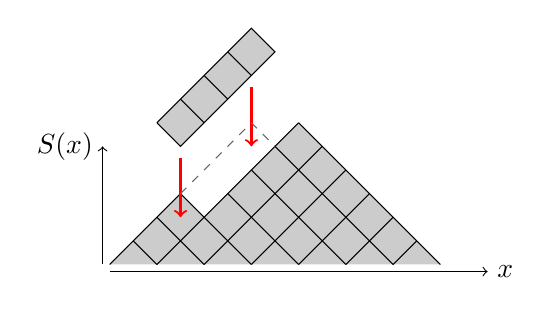
\begin{tikzpicture}[scale = .3]
\draw[->] (0, -.3) -- (16,-.3) node[right]{$x$};
\draw[->] (-.3,0) -- (-.3,5) node[left]{$S(x)$};
\fill[black!20] (0,0) -- (3,3) -- (4,2) -- (8,6) -- (14,0) ;
\draw (0,0) -- (3,3);
\draw (2,0) -- (8,6);
\draw (4,0) -- (9,5);
\draw (6,0) -- (10,4);
\draw (8,0) -- (11,3);
\draw (10,0) -- (12,2);
\draw (12,0) -- (13,1);
\draw (2,0) -- (1,1);
\draw (4,0) -- (2,2);
\draw (6,0) -- (3,3);
\draw (8,0) -- (5,3);
\draw (10,0) -- (6,4);
\draw (12,0) -- (7,5);
\draw (14,0) -- (8,6);

\draw[fill=black!20] (2,6) -- (3,5) -- (4,6) -- (5,7) -- (6,8) -- (7,9) --
					 (6,10) -- (3,7) -- (2,6);
\draw (4,6) -- (3,7);
\draw (5,7) -- (4,8);
\draw (6,8) -- (5,9);
%\draw (9,9) -- ()
\draw[thick, ->, red] (3,4.5) -- (3,2);
\draw[thick, ->, red] (6,7.5) -- (6,5);

\draw[dashed, black!60] (3,3) -- (6,6) -- (7,5);
\end{tikzpicture}
	\caption{\textbf{Near-maximal slope}. The single down step acts like a particle in the system. The 4 consecutive gates have the effect of moving the particle 3 sites to the right.}
	\label{fig:particle}
\end{figure}
Since gates can only act between a down step and an up step, these ``particles" follow a deterministic behavior for a given architecture and control the entropy growth in the circuit. 

Consider a series of consecutive gates with its first gate acting between sites $i$ and $i+1$ and its last gate between $j$ and $j+1$. Series of gates like this (called staircases) are discussed in Sec.~\ref{sec:stairs}. If there are no down steps in this region, the gate has no effect. If there is a single down step somewhere between sites $i$ and $j$, inclusive, that step gets moved to site $j+1$. More down steps will interact with each other but at the present we are only considering configurations with isolated down steps. 

Now consider an operator with the last non-identity contribution at a site between $i$ and $j$, inclusive. With probability 1, the series of gates in the last paragraph move the end of the operator to site $j+1$. This should demonstrate that operator ends and down step ``particles" have the same dynamics. 

The speed of the end of the operator is $v_B$. It is not immediately clear how the speed of the particle, call it $v_p$, should be related. If, in time $t$ the particle moves $v_pt$ sites, it has increased the \dots

\emph{Butterfly velocity of the two dynamics, operator and entanglement, is the same.}

\emph{Particles to not approach each other, so they remain uncorrelated.}